%%%%%%%%%%%%%%%%%%%%%%%%%%%%%%%%%%%%%%%%%%%%%%%%%%%%%%%%%%%%%%%%%%%%%%%%%%%%%%%%
%
% Template license:
% CC BY-NC-SA 3.0 (http://creativecommons.org/licenses/by-nc-sa/3.0/)
%
%%%%%%%%%%%%%%%%%%%%%%%%%%%%%%%%%%%%%%%%%%%%%%%%%%%%%%%%%%%%%%%%%%%%%%%%%%%%%%%%

%----------------------------------------------------------------------------------------
%	PACKAGES AND OTHER DOCUMENT CONFIGURATIONS
%----------------------------------------------------------------------------------------

\documentclass[
11pt, % The default document font size, options: 10pt, 11pt, 12pt
%oneside, % Two side (alternating margins) for binding by default, uncomment to switch to one side
%chapterinoneline,% Have the chapter title next to the number in one single line
spanish,
singlespacing, % Single line spacing, alternatives: onehalfspacing or doublespacing
%draft, % Uncomment to enable draft mode (no pictures, no links, overfull hboxes indicated)
%nolistspacing, % If the document is onehalfspacing or doublespacing, uncomment this to set spacing in lists to single
%liststotoc, % Uncomment to add the list of figures/tables/etc to the table of contents
%toctotoc, % Uncomment to add the main table of contents to the table of contents
parskip, % Uncomment to add space between paragraphs
%codirector, % Uncomment to add a codirector to the title page
headsepline, % Uncomment to get a line under the header
]{MastersDoctoralThesis} % The class file specifying the document structure



%----------------------------------------------------------------------------------------
%	INFORMACIÓN DE LA MEMORIA
%----------------------------------------------------------------------------------------

\thesistitle{Robot de exploración ambiental} % El títulos de la memoria, se usa en la carátula y se puede usar el cualquier lugar del documento con el comando \ttitle

% Nombre del posgrado, se usa en la carátula y se puede usar el cualquier lugar del documento con el comando \degreename
\posgrado{Carrera de Especialización en Sistemas Embebidos} 
%\posgrado{Carrera de Especialización en Internet de las Cosas} 
%\posgrado{Carrera de Especialización en Intelegencia Artificial}
%\posgrado{Maestría en Sistemas Embebidos} 
%\posgrado{Maestría en Internet de las cosas}

\author{Ing. Gonzalo Carreño} % Tu nombre, se usa en la carátula y se puede usar el cualquier lugar del documento con el comando \authorname

\director{Esp. Ing. Sergio Alberino (UTN.BA)} % El nombre del director, se usa en la carátula y se puede usar el cualquier lugar del documento con el comando \dirname
% El nombre del codirector si lo hubiera, se usa en la carátula y se puede usar el cualquier lugar del documento con el comando \codirname.  Para activar este campo se debe descomentar la opción "codirector" en el comando \documentclass, línea 23.

\juradoUNO{Nombre del jurado 1 (pertenencia)} % Nombre y pertenencia del un jurado se usa en la carátula y se puede usar el cualquier lugar del documento con el comando \jur1name
\juradoDOS{Nombre del jurado 2 (pertenencia)} % Nombre y pertenencia del un jurado se usa en la carátula y se puede usar el cualquier lugar del documento con el comando \jur2name
\juradoTRES{Nombre del jurado 3 (pertenencia)} % Nombre y pertenencia del un jurado se usa en la carátula y se puede usar el cualquier lugar del documento con el comando \jur3name

\ciudad{Ciudad Autónoma de Buenos Aires}

\fechaINICIO{marzo de 2023}
\fechaFINAL{noviembre de 2023}


\keywords{Sistemas embebidos, FIUBA} % Keywords for your thesis, print it elsewhere with \keywordnames


\begin{document}


\frontmatter % Use roman page numbering style (i, ii, iii, iv...) for the pre-content pages

\pagestyle{plain} % Default to the plain heading style until the thesis style is called for the body content


%----------------------------------------------------------------------------------------
%	RESUMEN - ABSTRACT 
%----------------------------------------------------------------------------------------

\begin{abstract}
\addchaptertocentry{\abstractname} % Add the abstract to the table of contents
%
%The Thesis Abstract is written here (and usually kept to just this page). The page is kept centered vertically so can expand into the blank space above the title too\ldots
\centering

\graphicspath{ {./Figures/} }

El presente trabajo describe un emprendimiento personal en el que se desarrolló un dispositivo robótico de exploración ambiental controlable a distancia con las funciones básicas de desplazamiento, medición y reporte de parámetros ambientales tales como presión, temperatura, humedad y luminosidad en una primera versión. No obstante, el sistema cuenta con una una arquitectura base robusta y flexible sobre la cual otros sensores pueden ser adaptados para poder tomar lecturas de otros parámetros ambientales, logrando por tanto brindar una solución que ayuda a incrementar la oferta en robots exploradores en la industria argentina pudiendo ser utilizados por ejemplo en aplicaciones de minería, agro, explotación de petróleo, etc. 
Para la implementación del trabajo se utilizaron conceptos y herramientas aprendidos en la especialización, tales como buenas prácticas en diseño y desarrollo de firmware, la utilización de sistemas operativos de tiempo real como plataforma de ejecución base, protocolos de comunicaciones para sistemas embebidos, y técnicas y frameworks de testing para asegurar la calidad del producto final. 


\end{abstract}

%----------------------------------------------------------------------------------------
%	CONTENIDO DE LA MEMORIA  - AGRADECIMIENTOS
%----------------------------------------------------------------------------------------

\begin{acknowledgements}
%\addchaptertocentry{\acknowledgementname} % Descomentando esta línea se puede agregar los agradecimientos al índice
\vspace{1.5cm}

Esta sección es para agradecimientos personales y es totalmente \textbf{OPCIONAL}.  

\end{acknowledgements}

%----------------------------------------------------------------------------------------
%	LISTA DE CONTENIDOS/FIGURAS/TABLAS
%----------------------------------------------------------------------------------------

\tableofcontents % Prints the main table of contents

\listoffigures % Prints the list of figures

\listoftables % Prints the list of tables


%----------------------------------------------------------------------------------------
%	CONTENIDO DE LA MEMORIA  - DEDICATORIA
%----------------------------------------------------------------------------------------

\dedicatory{\textbf{Dedicado a... [OPCIONAL]}}  % escribir acá si se desea una dedicatoria

%----------------------------------------------------------------------------------------
%	CONTENIDO DE LA MEMORIA  - CAPÍTULOS
%----------------------------------------------------------------------------------------

\mainmatter % Begin numeric (1,2,3...) page numbering

\pagestyle{thesis} % Return the page headers back to the "thesis" style

% Incluir los capítulos como archivos separados desde la carpeta Chapters

% Chapter 1

\chapter{Introducción general} % Main chapter title

\label{Chapter1} % For referencing the chapter elsewhere, use \ref{Chapter1} 
\label{IntroGeneral}

%----------------------------------------------------------------------------------------

% Define some commands to keep the formatting separated from the content 
\newcommand{\keyword}[1]{\textbf{#1}}
\newcommand{\tabhead}[1]{\textbf{#1}}
\newcommand{\code}[1]{\texttt{#1}}
\newcommand{\file}[1]{\texttt{\bfseries#1}}
\newcommand{\option}[1]{\texttt{\itshape#1}}
\newcommand{\grados}{$^{\circ}$}

%----------------------------------------------------------------------------------------

%\section{Introducción}

%----------------------------------------------------------------------------------------
\section{Motivación}

El presente proyecto es un emprendimiento personal que busca desarrollar un dispositivo robótico de exploración ambiental controlable a distancia con las funciones básicas de desplazamiento, medición y reporte de parámetros ambientales tales como presión, temperatura, humedad y luminosidad. 


%----------------------------------------------------------------------------------------

\section{Alcance y objetivos}

..

%----------------------------------------------------------------------------------------

\section{Estado del arte}

Los robots exploradores son dispositivos robotizados capaces de moverse de forma autónoma, y/o controlados a distancia, que han sido creados con el fin de reconocer y explorar un lugar o entorno donde una persona no pueda o deba acceder ya sea por motivos de capacidad, practicidad o seguridad. Por este motivo, en función de las necesidades de desplazamiento, existen diferentes sistemas de motricidad, como son por ejemplo, los bípedos, cuadrúpedos, con ruedas, tracción oruga, acuáticos/sumergibles, aéreos, etc. En cuanto a la forma de control, hay manejados por control remoto cableado o inalámbrico, habiendo equipos más sofisticados que gracias a aplicaciones de Inteligencia Artificial están preparados para desplazarse y tomar decisiones de forma autónoma. Algunos de los tipos de robots exploradores más conocidos son los espaciales, de minas, de rescate en catástrofes, de tuberías, acuáticos y/o submarinos, y de suelos.

\chapter{Introducción específica} % Main chapter title

\label{Chapter2}

%----------------------------------------------------------------------------------------
%	SECTION 1
%----------------------------------------------------------------------------------------
Todos los capítulos deben comenzar con un breve párrafo introductorio que indique cuál es el contenido que se encontrará al leerlo.  La redacción sobre el contenido de la memoria debe hacerse en presente y todo lo referido al proyecto en pasado, siempre de modo impersonal.

\section{Requerimientos}
...

\section{Tecnologias de hardware utilizadas}

...

\section{Tecnologias de software utilizadas} 

... 
\chapter{Diseño e implementación} % Main chapter title

\label{Chapter3} % Change X to a consecutive number; for referencing this chapter elsewhere, use \ref{ChapterX}

\definecolor{mygreen}{rgb}{0,0.6,0}
\definecolor{mygray}{rgb}{0.5,0.5,0.5}
\definecolor{mymauve}{rgb}{0.58,0,0.82}

%%%%%%%%%%%%%%%%%%%%%%%%%%%%%%%%%%%%%%%%%%%%%%%%%%%%%%%%%%%%%%%%%%%%%%%%%%%%%
% parámetros para configurar el formato del código en los entornos lstlisting
%%%%%%%%%%%%%%%%%%%%%%%%%%%%%%%%%%%%%%%%%%%%%%%%%%%%%%%%%%%%%%%%%%%%%%%%%%%%%
\lstset{ %
  backgroundcolor=\color{white},   % choose the background color; you must add \usepackage{color} or \usepackage{xcolor}
  basicstyle=\footnotesize,        % the size of the fonts that are used for the code
  breakatwhitespace=false,         % sets if automatic breaks should only happen at whitespace
  breaklines=true,                 % sets automatic line breaking
  captionpos=b,                    % sets the caption-position to bottom
  commentstyle=\color{mygreen},    % comment style
  deletekeywords={...},            % if you want to delete keywords from the given language
  %escapeinside={\%*}{*)},          % if you want to add LaTeX within your code
  %extendedchars=true,              % lets you use non-ASCII characters; for 8-bits encodings only, does not work with UTF-8
  %frame=single,	                % adds a frame around the code
  keepspaces=true,                 % keeps spaces in text, useful for keeping indentation of code (possibly needs columns=flexible)
  keywordstyle=\color{blue},       % keyword style
  language=[ANSI]C,                % the language of the code
  %otherkeywords={*,...},           % if you want to add more keywords to the set
  numbers=left,                    % where to put the line-numbers; possible values are (none, left, right)
  numbersep=5pt,                   % how far the line-numbers are from the code
  numberstyle=\tiny\color{mygray}, % the style that is used for the line-numbers
  rulecolor=\color{black},         % if not set, the frame-color may be changed on line-breaks within not-black text (e.g. comments (green here))
  showspaces=false,                % show spaces everywhere adding particular underscores; it overrides 'showstringspaces'
  showstringspaces=false,          % underline spaces within strings only
  showtabs=false,                  % show tabs within strings adding particular underscores
  stepnumber=1,                    % the step between two line-numbers. If it's 1, each line will be numbered
  stringstyle=\color{mymauve},     % string literal style
  tabsize=2,	                   % sets default tabsize to 2 spaces
  title=\lstname,                  % show the filename of files included with \lstinputlisting; also try caption instead of title
  morecomment=[s]{/*}{*/}
}


%----------------------------------------------------------------------------------------
%	SECTION 1
%----------------------------------------------------------------------------------------

Esta sección presenta los detalles técnicos del diseño e implementación de las diferentes funcionalidades del producto, la arquitectura hardware y software, y finalmente la interfaz de usuario para el control y reporte de las operaciones del robot.

El proyecto fue realizado siguiendo una metodologia basada en crear un prototipo funcional con una arquitectura escalable que cumpla con alcance basico especificado en el plan de proyecto, y una vez conseguido agregar en lo posible y de acuerdo a la capacidad, funcionalidades adicionales.
De esta forma, una vez que se logro el alcance basico, considerado como la version v1.0 del producto, se continuo con el desarrollo y se agrego la funcionalidad adicional de control inalambrico por medio de un joystick, en lo que se considera la version v2.0 del mismo.

En las siguientes sub secciones se detallan los detalles del disenio e implementacion realizados tanto para el cumplimiento con el alcance basico como con el agregado de la funcionalidad adicional que comprende el robot en su version final.



\section{Arquitectura de software del sistema}


\subsection{Perspectiva global}

A continuacion podemos apreciar la arquitectura macro del sistema.

\begin{center}
  \includegraphics[scale=0.75]{software/arquitectura_software_global}
    \captionof{figure}{Arquitectura global.}
    \label{fig:arquitectura_software_global}

\end{center}



\subsection{Disenio de componentes y servicios}


Con el fin de poder lograr una arquitectura de software modular, se implementaron diferentes componentes software y servicios que abstraen el acceso a los modulos de hardware (explicados en la siguiente seccion) y permitieron un escalamiento facil de funcionalidades en la expancion de las funcionalidades del robot entre su version basica y su version final.

Los componentes y servicios de software del Robot en la version v1 son los siguientes:

\begin{enumerate}	
	\item Componentes de software del Robot
	\begin{enumerate}			
		\item main-core: orquesta las diferentes tareas desde las que se invocan los demas componentes de software.
		\item Measuring Service: abstrae el acceso a los modulos de medicion de temperatura, humedad, presion y luminosidad.
		\item Measuring State: mantiene el estado de cada uno de los parametros ambientales medidos.
		\item Robot Position State: mantiene el estado del movimiento actual del robot.
		\item ADC Service: abstrae el acceso a los modulos que hacen uso de los canales que requieren conversiones ADC (Analogico/Digital), como el joystick analogico y el fotoresistor. 
		\item Motors Service: abstrae el acceso al modulo de control de motores.
		\item Display Service: abstrae el acceso al modulo de control del display mediante Ic2.
		\item Joystick Service: abstrae el acceso al modulo de control del joystick.
	\end{enumerate}	
	\item Servicios (tareas) del Robot
	\begin{enumerate}				
		\item Display Task	
		\item Measuring Task		
		\item Joystick Task
		\item Motors Task		
	\end{enumerate}			
\end{enumerate}		


Luego de expandir su funcionalidad, los componentes y servicios de software se separaron fisicamente en el hardware del robot y el del joystick, agregandose ademas los necesarios para la comunicacion inalambrica, quedando de la siguiente manera:

\begin{enumerate}	
	\item Componentes de software del Robot
	\begin{enumerate}			
		\item main-core
		\item Measuring Service	
		\item Measuring State
		\item Robot Position State
		\item ADC Service
		\item Motors Service
		\item WIFI Service
		\item UDP Service	
	\end{enumerate}	
	\item Servicios (tareas) del Robot
	\begin{enumerate}				
		\item Measuring Task		
		\item Motors Task	
		\item UDP Server Task
	\end{enumerate}			
\end{enumerate}		


\begin{enumerate}	
	\item Componentes de software del Joystick
	\begin{enumerate}			
		\item main-core
		\item Measuring State
		\item Robot Position State
		\item UDP Service	
	\end{enumerate}	
	\item Servicios (tareas) del Joystick
	\begin{enumerate}				
		\item Display Task		
		\item Joystick Task	
		\item UDP Server Task
	\end{enumerate}			
\end{enumerate}		

\section{Implementacion de los modulos}

Los macro componentes de hardware presentes en la arquitectura de la version 2 son el robot y el joystick.
Internamente se disenio su micro arquitectura de forma modular, de forma tal que se permita la adaptacion de los diferentes componentes de forma independiente.
El conexionado de cada uno de ellos puede apreciase a continuacion:
(conexionado de los modulos)

La integracion de los mismos se realizo mediante el disenio y contruccion de una placa integradora base que permite


La arquitectura de software del sistema esta compuesta por los siguientes modulos:
- servicio de control del display
- servicio de control de los motores DC
- servicio de control de los sensores
- servicio de control del joystick
- servicio de comunicacion inalambrica via WIFI



\subsection{Medición de temperatura y humedad}

Para el desarrollo de este prototipo se utilizó la biblioteca de código ESP-IDF-Lib Components Library \cite{esp_idf_lib_website} que provee el soporte para gestionar el DHT11. Para acceder a las lecturas del dispositivo se abstrajo el mismo mediante el componente Measuring Service, el cual es invocado en cada iteracion del 
A continuación se puede apreciar el conexionado del prototipo en la figura \ref{fig:conexionado_dht11} y los detalles de sus pines en la tabla \ref{tab:conexionado_dht11}.

\vspace{0.5cm}
\begin{table}[h]
\centering
\caption[Conexionado DHT11]{Conexionado DHT11}
\begin{tabular}{l c }
\toprule
\textbf{Nombre lógico} &  \textbf{Pin GPIO}\\
\midrule
 Pin DHT11  & 4  \\
\bottomrule
\hline
\end{tabular}
\label{tab:conexionado_dht11} 
\end{table}
 
\vspace{0.5cm}   
\begin{center}
  \includegraphics[scale=1]{schematics/conexionado_dht11}
    \captionof{figure}{Circuito del conexionado DHT11.}
    \label{fig:conexionado_dht11}
\end{center}



\subsection{Medición de presión}
Para el desarrollo de este prototipo se utilizó el framework ESP-IDF y la biblioteca de código ESP-IDF Components que provee el soporte para gestionar el BMP280. A continuación se puede apreciar el conexionado del prototipo en la figura \ref{fig:conexionado_bmp280} y los detalles de sus pines en la tabla \ref{tab:conexionado_bmp280}.

\vspace{0.5cm}    
\begin{table}[h]
\centering
\caption[Conexionado BMP280]{Conexionado BMP280}
\begin{tabular}{l c }
\toprule
\textbf{Nombre lógico} &  \textbf{Pin GPIO}\\
\midrule
 BMP SDA & 18 \\
 BMP280 SCL & 19  \\
\bottomrule
\hline
\end{tabular}
\label{tab:conexionado_bmp280} 
\end{table}
    
\vspace{0.5cm}    
\begin{center}
  \includegraphics[scale=1]{schematics/conexionado_bmp280}
    \captionof{figure}{Conexionado BMP280.}
    \label{fig:conexionado_bmp280}
\end{center}




\subsection{Medición de valor de luminosidad}
Para el desarrollo de este prototipo se utilizó el siguiente conexionado y la biblioteca de código ADC provista por ESP-IDF. A continuación se puede apreciar el conexionado del prototipo en la figura \ref{fig:conexionado_fotoresistor} y los detalles de sus pines en la tabla \ref{tab:conexionado_fotoresistor}.

\vspace{0.5cm}    
\begin{table}[h]
\centering
\caption[Conexionado fotorresistor]{Conexionado fotorresistor}
\begin{tabular}{l c c}
\toprule
\textbf{Nombre lógico} & \textbf{Pin ADC} & \textbf{Pin GPIO}\\
\midrule
ADC Fot pin & channel 0 - unit 2 & 4\\
\bottomrule
\hline
\end{tabular}
\label{tab:conexionado_fotoresistor}
\end{table}


\vspace{0.5cm}
\begin{center}
  \includegraphics[scale=1]{schematics/conexionado_fotoresistor}
    \captionof{figure}{Conexionado fotorresistor.}
    \label{fig:conexionado_fotoresistor}
    
\end{center}

\subsection{Control del joystick analogico}
Para el desarrollo de este prototipo se utilizó el siguiente conexionado y la biblioteca de código ADC provista por ESP-IDF. A continuación se puede apreciar el conexionado del prototipo en la figura \ref{fig:conexionado_joystick} y los detalles de sus pines en la tabla \ref{tab:conexionado_joystick}.


\vspace{0.5cm}
\begin{table}[h]
\centering
\caption[Conexionado joystick]{Conexionado joystick}
\begin{tabular}{l c c}
\toprule
\textbf{Nombre lógico} & \textbf{Pin ADC} & \textbf{Pin GPIO}\\
\midrule
ADC X & channel 1 - unit 2 & 0 \\
ADC Y & channel 7 - unit 1 & 35 \\
\bottomrule
\hline
\end{tabular}
\label{tab:conexionado_joystick}
\end{table}

\vspace{0.5cm}

\begin{center}
  \includegraphics[scale=1]{schematics/conexionado_joystick}
    \captionof{figure}{Conexionado joystick.}
    \label{fig:conexionado_joystick}
    

\end{center}

\subsection{Control del display}
 
\begin{center}
  \includegraphics[scale=1]{schematics/conexionado_display}
    \captionof{figure}{Conexionado display.}
    \label{fig:conexionado_display}

\end{center}

\subsection{Control de motores DC}


\begin{center}
  \includegraphics[scale=1]{schematics/conexionado_motores}
    \captionof{figure}{Conexionado motores.}
    \label{fig:conexionado_motores}

\end{center}

\subsection{Control de la red WIFI}
\subsection{Gestion de la  de la comunicacion sockets UDP}



\section{Arquitectura de hardware}


\subsection{Conexionado logico }


\begin{center}
  \includegraphics[scale=0.75]{schematics/conexionado_completo_robot}
    \captionof{figure}{Conexionado del robot.}
    \label{fig:conexionado_completo_robot}
\end{center}



\begin{center}
  \includegraphics[scale=0.75]{schematics/conexionado_completo_joystick}
    \captionof{figure}{Conexionado del joystick.}
    \label{fig:conexionado_completo_joystick}
\end{center}


\subsection{Conexionado fisico }




% Chapter Template

\chapter{Ensayos y resultados} % Main chapter title

\label{Chapter4} % Change X to a consecutive number; for referencing this chapter elsewhere, use \ref{ChapterX}

%----------------------------------------------------------------------------------------
%	SECTION 1
%----------------------------------------------------------------------------------------
Esta sección presenta los diferentes prototipos realizados para determinar la viabilidad de cada una de las funcionalidades provistas, la metodología de desarrollo, testing y, finalmente, los entregables finales del trabajo.

\section{Proceso de desarrollo y aseguramiento de calidad}
\label{sec:pruebasHW}

Para el proceso de desarrollo se realizaron pruebas de concepto de las diferentes funcionalidades utilizando como materiales la bibliografía encontrada en Internet, las hojas de datos y los ejemplos de código provistos por el SDK y bibliotecas empleadas. Una vez logrado el objetivo funcional de cada componente, se optimizó y encapsuló cada módulo para ser integrado de manera individual a un prototipo integrador sin afectar el funcionamiento de cualquier otro módulo.
De esta manera, se desarrolló un prototipo integrador como la sumatoria de todos los módulos de forma incremental, probándose por regresión que los módulos ya integrados previamente siguieran funcionando de forma óptima.

Una vez logrado el prototipo integrador, con todas las funcionalidades de la versión v1.0, se procedió a expandir el hardware para crear la versión v2.0. Para ello, se extrajeron los módulos de joystick y display, que posteriormente se agregarían al sistema embebido del joystick, y se incorporaron los módulos de conectividad UDP sobre Wi-Fi.

Tras lograr la versión v2.0 se repite el proceso de control de calidad de los diferentes módulos ya integrados.

En las siguientes secciones, se detallan las diferentes pruebas realizadas.

\section{Verificación técnica de los diferentes módulos}


Todos los módulos fueron probados mediante una inspección visual durante el proceso de pruebas de concepto.


\subsection{Verificación del módulo de joystick}
Se verificó visualmente que los valores del joystick analógico puedan ser leídos apropiadamente, y que sean representativos y relevantes con la dirección del movimiento de la palanca sobre sus coordenadas X e Y.

\subsection{Verificación del módulo de control del display}
Se verificó visualmente que el display mostraba los caracteres programados en la prueba de concepto con una intensidad de luz aceptable para poder leerlos apropiadamente.


\subsection{Verificación del módulo de control de motores}
Se verificó visualmente que individualmente el motor pudiera girar en ambos sentidos. Luego, al implementarse los cuatro motores con sus ruedas, se probó que se puedan realizar los giros en todas las direcciones.

\subsection{Verificación del módulo de medición de temperatura y humedad}
Se verificó visualmente que los valores obtenidos por el sensor DHT11 coincidieran con los esperados en relación a la temperatura en el interior del lugar de experimentación y que la humedad detectada se aproximara a los valores resportados por Google.

\subsection{Verificación del módulo de medición de presión atmosférica}
Se verificó visualmente que el valor obtenido por el sensor BMP280 fuera cercano a lo esperado en relación al valor reportado por Google.


\subsection{Verificación del módulo de medición de luminosidad}
Se verificó visualmente que los valores obtenidos del fotorresistor, una vez transformados a valores absolutos porcentuales, reflejaban el nivel de luminosidad ambiental del interior del lugar de experimentación.


\subsection{Verificación del módulo de comunicación UTP sobre Wi-Fi}
Por medio de dos programas UDP, uno cliente y uno servidor, se probó el establecimiento de la comunicación UDP entre dos ESP32. Posteriormente, se incorporó el servicio de comunicaciones UDP en el robot, y desde el programa cliente se enviaban las acciones que representaban las direcciones del movimiento (FORWARD, BACKWARD, LEFT, RIGHT). Se observó visualmente cómo el robot giraba sus ruedas en función de los comandos enviados. Finalmente, se incorporó el módulo de comunicaciones en el joystick y activó el desplazamiento en cada una de sus direcciones. El robot se desplazó correctamente en respuesta a cada comando recibido.


\section{Pruebas funcionales y validación del producto}

El proceso de validación y pruebas del producto, se realizó comparando el resultado obtenido con los valores esperados en el alcance del proyecto.

Para la medición de temperatura, humedad y presión, se utilizó el anemómetro digital de la figura \ref{fig:anemometro}, mientras que para la validación de la medición de luminosidad ambiental se utilizó la observación visual.

Las pruebas realizadas fueron las siguientes:
\begin{itemize}
	\item Prueba y validación del módulo de visualización de display.
	\item Prueba y validación del módulo de medición de temperatura y humedad.
	\item Prueba y validación del módulo de medición de presión atmosférica.
	\item Prueba y validación del módulo de medición de luminosidad ambiental.
	\item Prueba y validación del control y desplazamiento del robot.
\end{itemize}

En las siguientes secciones se presentan las diferentes pruebas funcionales realizadas sobre el producto.


\subsection{Prueba y validación del módulo de visualización de display}

Se verificó el funcionamiento del display visualizando las lecturas de los valores censados y transmitidos por el robot. Se controló que:

\begin{itemize}
	\item Las lecturas sean nítidas y entendibles.
	\item Las unidades de medida están presentes.
	\item Haya un detalle de lo que se está midiendo acompañando las lecturas y la unidad de medida.
	\item El nivel de luminosidad sea óptimo para permitir la lectura independientemente de la iluminación ambiental.
	\item Se presentan las lecturas de todos los valores observados.
\end{itemize}


A continuación, se pueden apreciar algunas fotografías tomadas durante el proceso de experimentación:

\begin{center}
\includegraphics[scale=0.094]{demo_product/DisplayNoche}
  \captionof{figure}{Visualización del display en la oscuridad.}
  \label{fig:DisplayNoche}
\end{center}


En la siguiente sección pueden encontrarse los videos en los que se puede apreciar el funcionamiento del display durante el día \cite{Demo_Mediciones} y en la oscuridad \cite{Demo_Display_Oscuridad}.

\subsection{Prueba y validación del módulo de medición de temperatura y humedad}

Se compararon los valores medidos por el módulo de medición de temperatura y humedad basado en el sensor DHT11 con los obtenidos a través de un dispositivo de medición de temperatura y humedad. Se realizó la medición en diferentes contextos:

\begin{itemize}
	\item En el interior de una casa.
	\item En el exterior, durante el día.
\end{itemize}

En la siguiente tabla se pueden apreciar los resultados.

\begin{table}[h]
\centering
\caption[Resultados de mediciones de temperatura y humedad]{Resultados de mediciones de temperatura y humedad}
\begin{tabular}{l c c c c}
\toprule
\textbf{Contexto} & \textbf{Temp. Robot} & \textbf{Temp. Ref.} & \textbf{Hume. Robot}  & \textbf{Hume. Ref.}\\
\midrule
Interior & 22,0 & 23,6 & 44,0 - 45,0 & 58,5 \\
Exterior (día) & 17,0  & 14,0 & 47,0 - 53,0 & 62,9 - 64,0 \\
Exterior (noche) & - & - & - & - \\
\bottomrule
\hline
\end{tabular}
\end{table}

A continuación, se pueden apreciar algunas fotografías tomadas durante el proceso de experimentación:

\begin{center}
\includegraphics[scale=0.094]{demo_product/humedad_interior_retouched}
  \captionof{figure}{Medición de humedad en el interior.}
  \label{fig:humedad_interior}
\end{center}

\begin{center}
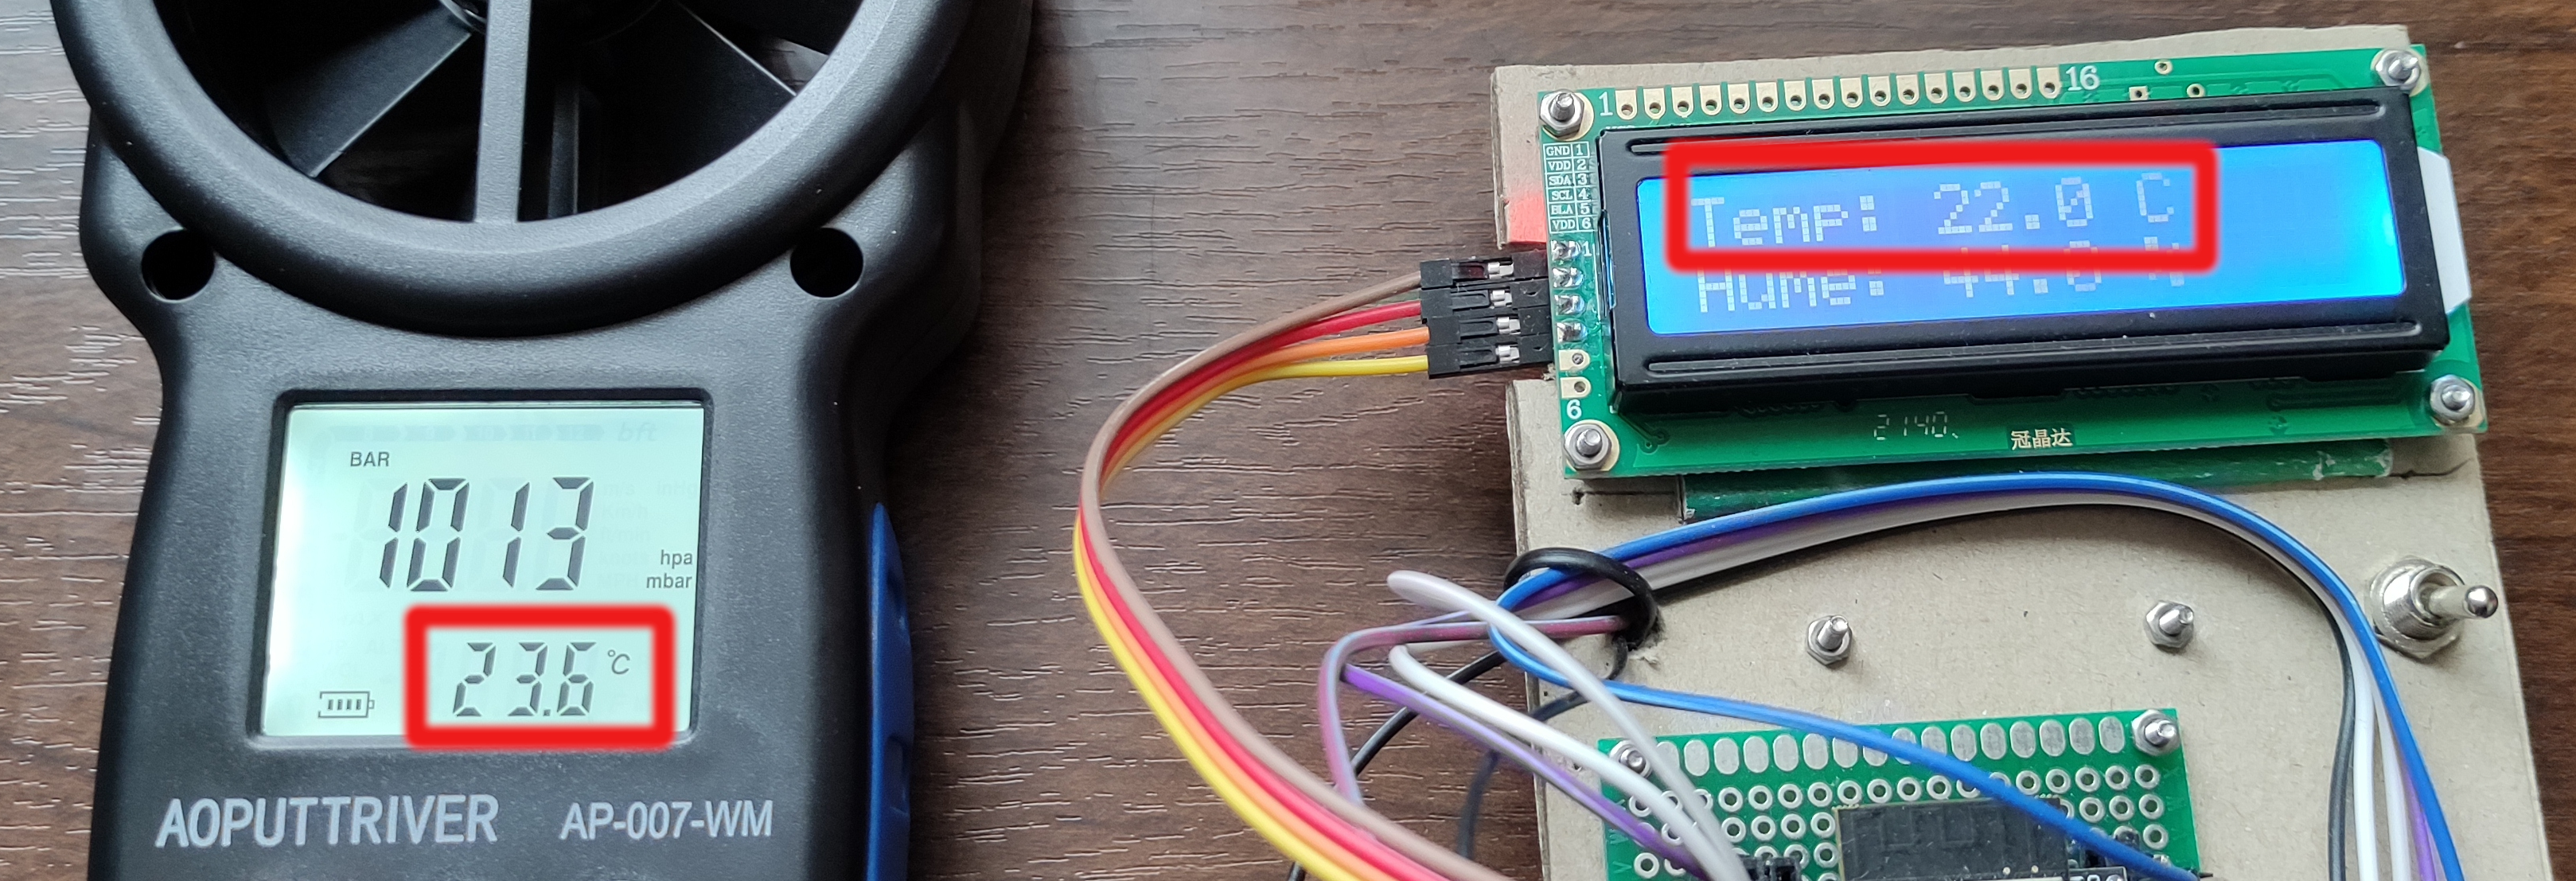
\includegraphics[scale=0.1]{demo_product/temp_interior_retouched}
  \captionof{figure}{Medición de temperatura en el interior.}
  \label{fig:humedad_interior}
\end{center}


\begin{center}
\includegraphics[scale=0.125]{demo_product/humedad_exterior_retouched}
  \captionof{figure}{Medición de humedad en el exterior.}
  \label{fig:humedad_interior}
\end{center}

\begin{center}
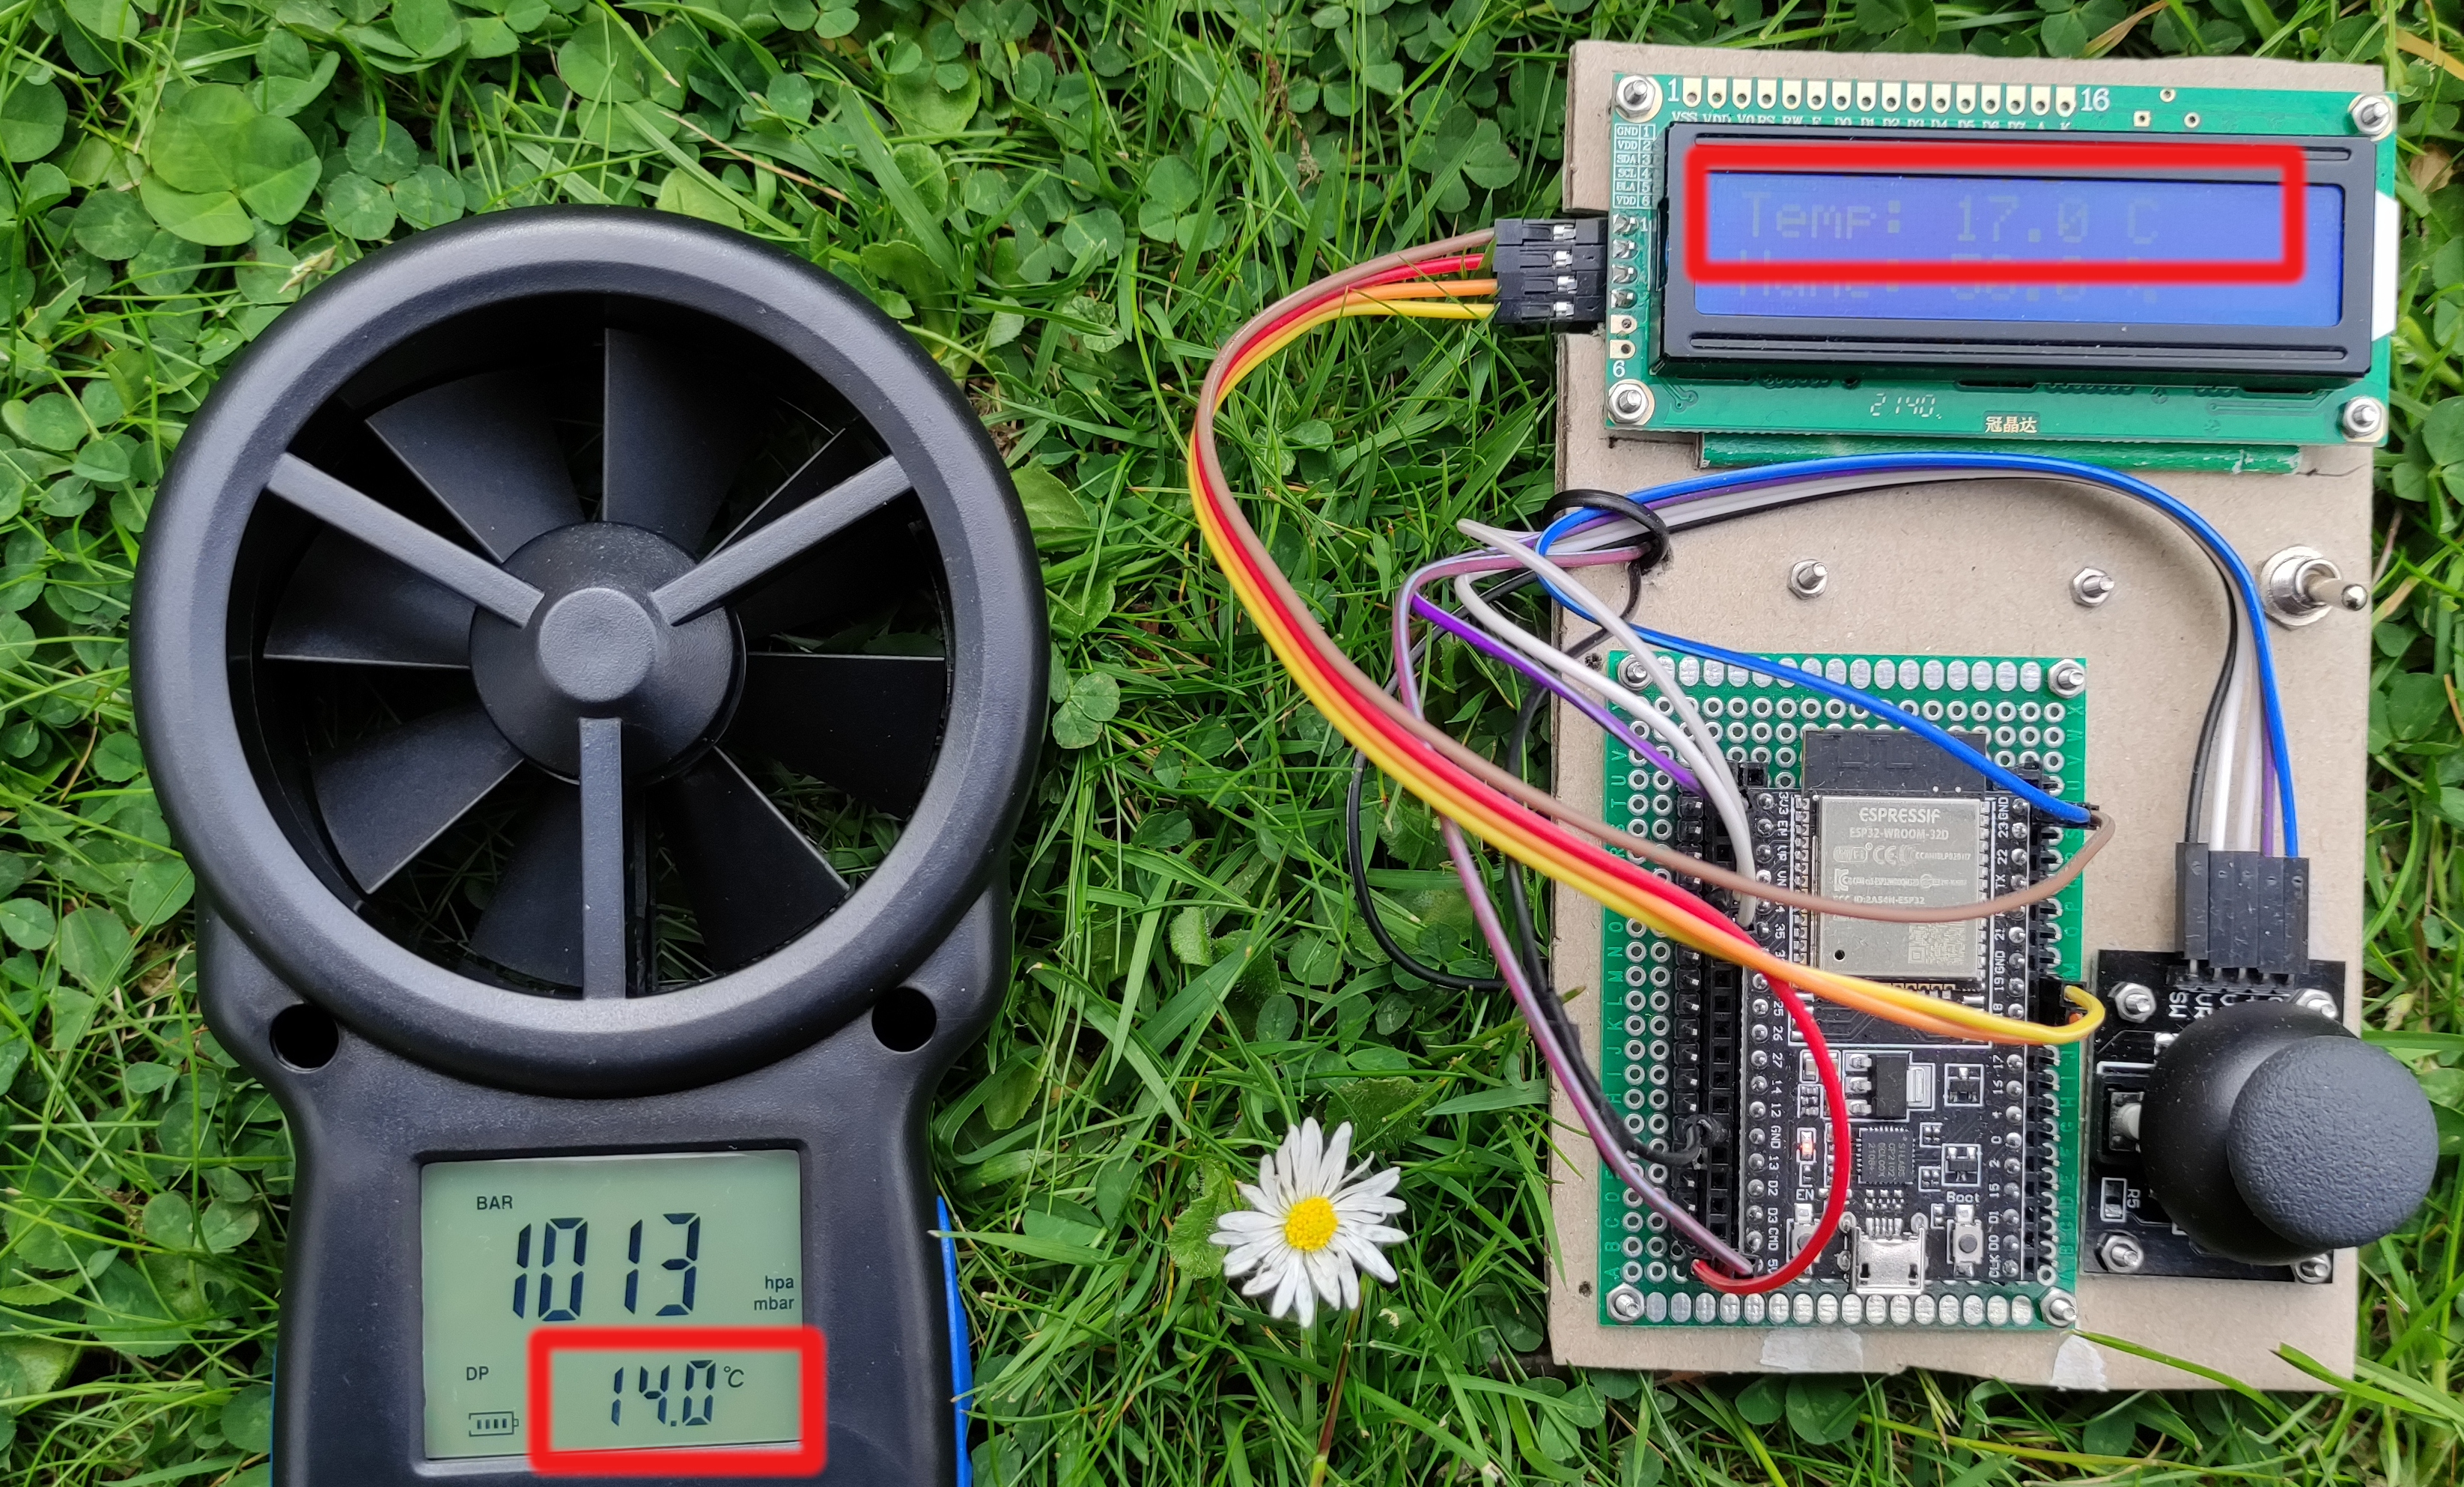
\includegraphics[scale=0.1]{demo_product/temp_exterior_dia_retouched}
  \captionof{figure}{Medición de temperatura en el exterior.}
  \label{fig:humedad_interior}
\end{center}

En la siguiente sección puede encontrarse el video que muestra el funcionamiento del módulo de mediciones, en el que se aprecia el funcionamiento del módulo de medición de temperatura y humedad \cite{Demo_Mediciones}.

\subsection{Prueba y validación del módulo de medición de presión atmosférica}

Se compararon los valores medidos por el módulo de medición de presión basado en el sensor BMP280 con los obtenidos a través de un dispositivo manómetro digital. Las mediciones se realizaron en el interior de la vivienda en dos días distintos.

En la siguiente tabla pueden apreciarse los resultados obtenidos:

\begin{table}[h]
\centering
\caption[Resultados de mediciones de presión ambiental.]{Resultados de mediciones de presión ambiental.}
\begin{tabular}{l c c}
\toprule
\textbf{Contexto} & \textbf{Presión. Robot} & \textbf{Presión. Ref.} \\
\midrule
Día 1 & 1013 & 1018,9 \\
Día 2 & 1003,9 & 998 \\
\bottomrule
\hline
\end{tabular}
\end{table}

\begin{center}
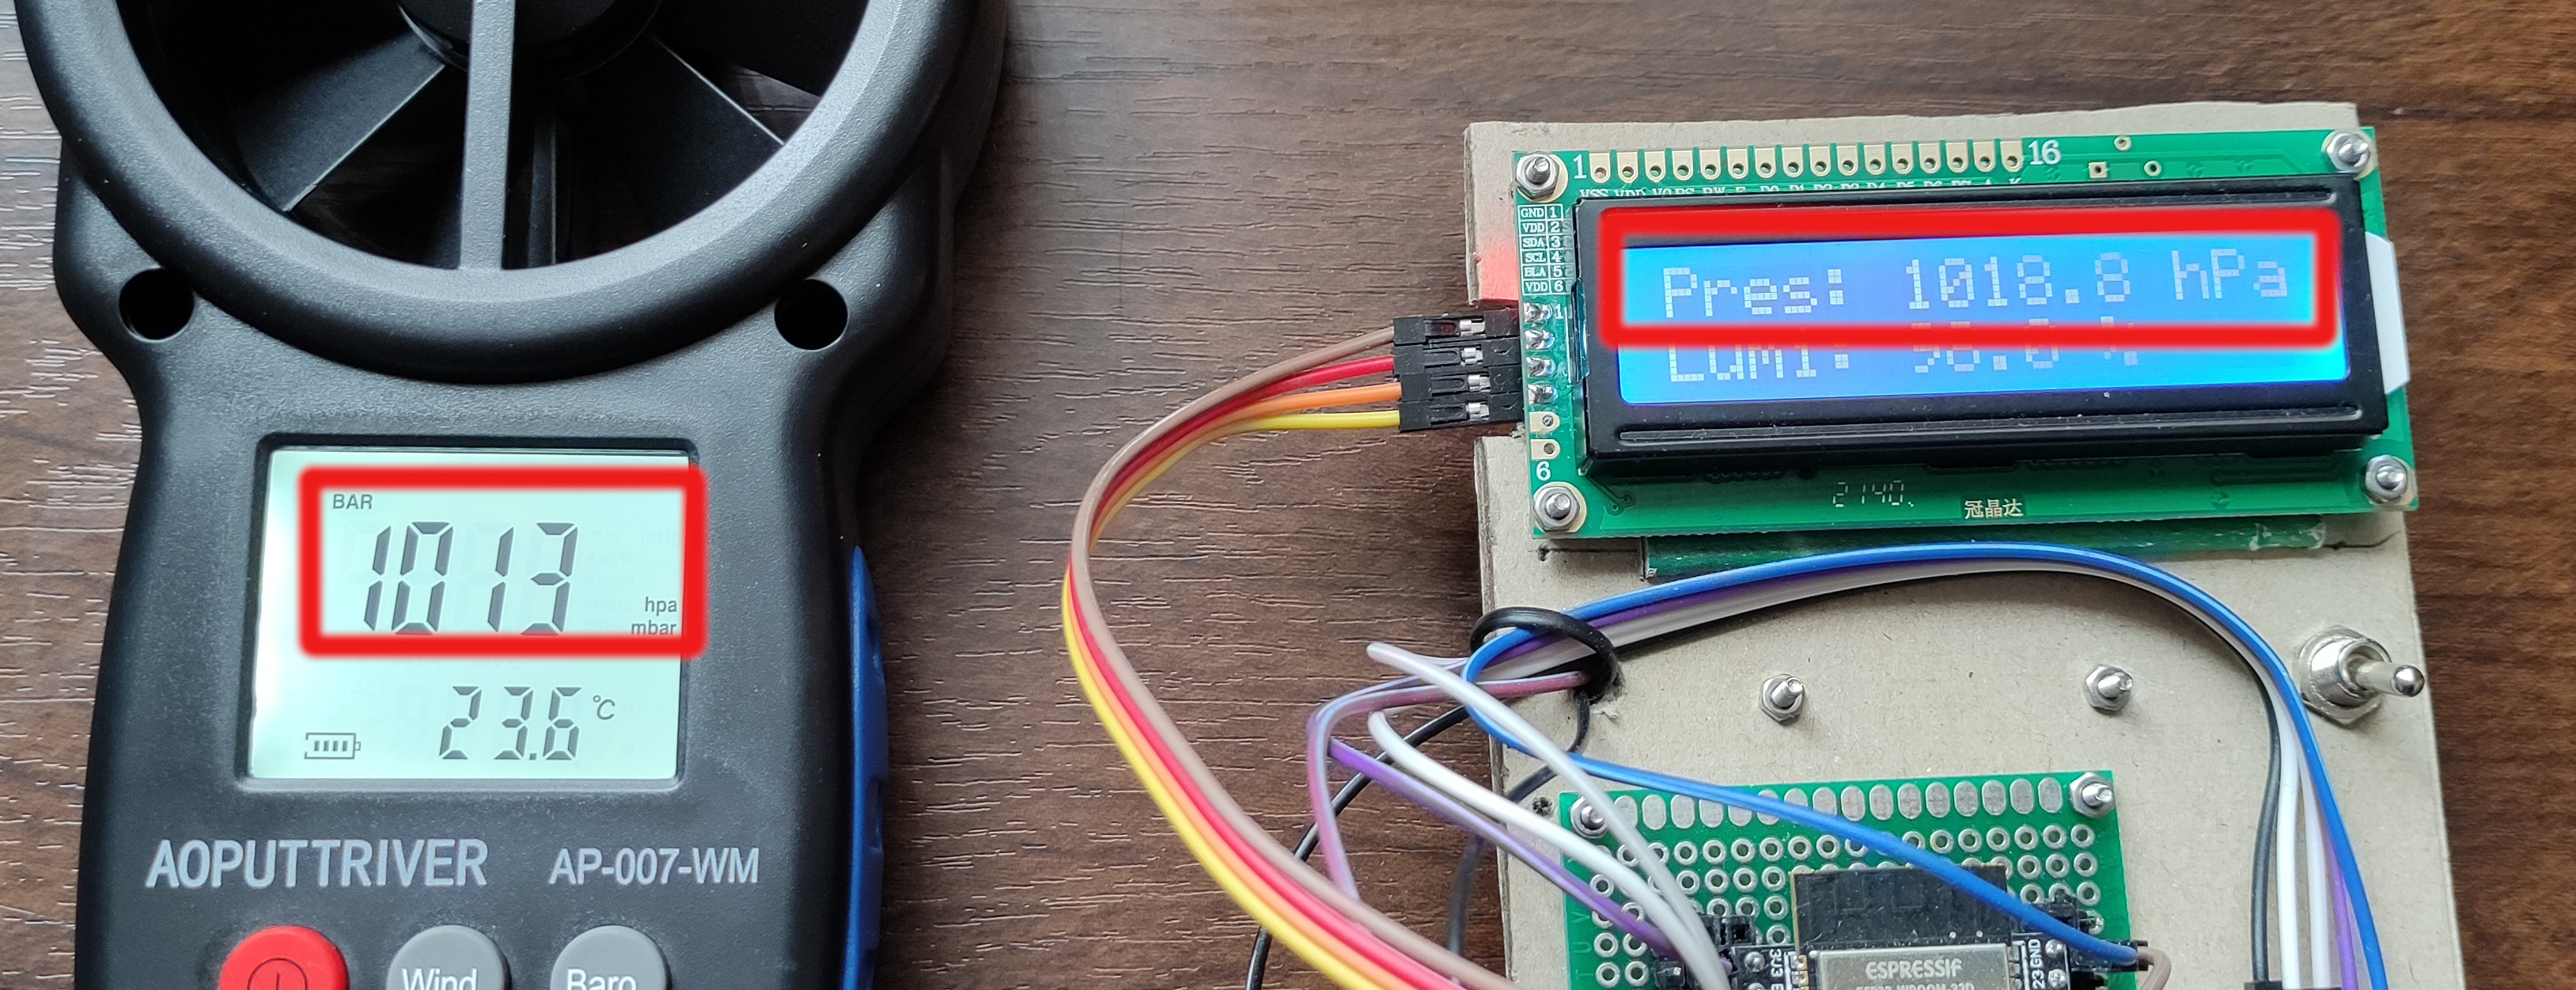
\includegraphics[scale=0.1]{demo_product/presion_interior_retouched}
  \captionof{figure}{Medición de presión atmosférica en el interior.}
  \label{fig:humedad_interior}
\end{center}

\begin{center}
\includegraphics[scale=0.1]{demo_product/presion_exterior_retouched}
  \captionof{figure}{Medición de presión atmosférica en el exterior.}
  \label{fig:humedad_interior}
\end{center}


En la siguiente sección puede encontrarse el video que muestra el funcionamiento del módulo de mediciones, en el que se aprecia el funcionamiento del módulo de medición de presión atmosférica \cite{Demo_Mediciones}.

\subsection{Prueba y validación del módulo de medición de luminosidad ambiental}

Se compararon los valores medidos por el módulo de medición de luminosidad basado en un fotorresistor percibidos por el ojo humano sin utilizar ningún dispositivo de medición. Se realizó la medición en diferentes escenarios:

\begin{itemize}
	\item En exteriores durante el día con luz ambiental.
	\item En interiores con luz ambiental.
	\item En interiores a oscuras.
\end{itemize}

Los resultados mostraron que los valores porcentuales indicados por el módulo de medición de luminosidad son consistentes con los niveles de luz detectados por el ojo humano. En las figuras \ref{fig:DisplayLuminosidadExteriorDia}, \ref{fig:DisplayLuminosidadInteriorDia} y \ref{fig:DisplayLuminosidadInteriorNoche} pueden apreciarse los resultados de las mediciones.

\begin{center}
\includegraphics[scale=0.8]{demo_product/DisplayLuminosidadExteriorDia}
  \captionof{figure}{Medición de luminosidad ambiental en el exterior durante el día.}
  \label{fig:DisplayLuminosidadExteriorDia}
\end{center}

\begin{center}
\includegraphics[scale=0.23]{demo_product/DisplayLuminosidadInteriorDia}
  \captionof{figure}{Medición de luminosidad ambiental en interiores durante el día.}
  \label{fig:DisplayLuminosidadInteriorDia}
\end{center}

\begin{center}
\includegraphics[scale=0.82]{demo_product/DisplayLuminosidadInteriorNoche}
  \captionof{figure}{Medición de luminosidad ambiental en interiores durante la noche.}
  \label{fig:DisplayLuminosidadInteriorNoche}
\end{center}

En la siguiente sección puede encontrarse el video que muestra el funcionamiento del módulo de mediciones, en el que se aprecia el funcionamiento del módulo de medición de luminosidad ambiental \cite{Demo_Mediciones}.

\subsection{Prueba y validación del control y desplazamiento del robot}

Se verificó el control del desplazamiento del robot de forma visual por medio de accionar el joystick en las diferentes coordenadas (X;Y) y se controló que:

\begin{itemize}
	\item La dirección del movimiento del robot sea acorde al accionamiento del joystick.
	\item El tiempo de respuesta en el movimiento del robot y tras el accionar del joystick sea mínimo, permitiendo una buena experiencia de usuario.
\end{itemize}

En la siguiente sección pueden encontrarse los videos \cite{Demo_Control_Movimiento_1} y \cite{Demo_Control_Movimiento_2} evidenciando la demostración de este experimento.



\section{Videos del producto durante el ensamblado y experimentación}

En las siguientes subsecciones se listan los videos realizados durante el proceso de demostración del producto funcionando así como los grabados casualmente durante armado y prototipado del mismo.


\subsection{Videos demostrativos del producto final}

Los experimentos realizados para evidenciar el cumplimiento con los requerimientos funcionales del producto son los siguientes:
\begin{itemize}
	\item Demo - Hardware del producto \cite{Demo_Hardware}.
	\item Demo - Comunicación Wi-Fi \cite{Demo_ComWifi}.
	\item Demo - Control de movimiento de las ruedas \cite{Demo_Control_Movimiento_1}.
	\item Demo - Medición y visualización de parámetros ambientales \cite{Demo_Mediciones}.
	\item Demo - Control de desplazamiento en un circuito \cite{Demo_Control_Movimiento_2}.
	\item Demo - Visualización del Display en la oscuridad \cite{Demo_Display_Oscuridad}.
	
\end{itemize}


\subsection{Videos durante el prototipado y ensamblado del robot}

\begin{itemize}
	\item Prototipado Robot v1 - Ensamblado (1) \cite{Prototipado_Ensamblado_1}.	
	\item Prototipado Robot v1 - Ensamblado (2) \cite{Prototipado_Ensamblado_2}.
	\item Prototipado Robot v1 - Ensamblado (3) \cite{Prototipado_Ensamblado_3}.
	\item Prototipado Robot v1 - Ensamblado (4) \cite{Prototipado_Ensamblado_4}.
	\item Prototipado Robot v2 - Comunicación Joystick Robot (1) \cite{Prototipado_Comunicacion_JoystickRobot1}.
	\item Prototipado Robot v2 - Comunicación Joystick Robot (2) \cite{Prototipado_Comunicacion_JoystickRobot2}.
	\item Prototipado Desplazamiento (alimentación USB) \cite{Prototipado_Desplazamiento_USB}.
	\item Prototipado Desplazamiento (alimentación por pilas) \cite{Prototipado_Desplazamiento_Pilas}.

\end{itemize}




\section{Documentación del producto }

Se desarrolló la documentación del producto compuesta de los siguientes entregables
\begin{itemize}
	\item Documentación técnica \cite{Robot_Tecnical_doc}.
	\item Manual de usuario \cite{Robot_User_manual}.
\end{itemize}











 
% Chapter Template

\chapter{Conclusiones} % Main chapter title

\label{Chapter5} % Change X to a consecutive number; for referencing this chapter elsewhere, use \ref{ChapterX}


%----------------------------------------------------------------------------------------

%----------------------------------------------------------------------------------------
%	SECTION 1
%----------------------------------------------------------------------------------------

% \begin{itemize}\item ¿Cuál es el grado de cumplimiento de los requerimientos?
En el presente trabajo se ha implementado un robot de exploración ambiental cumpliendo con todos los requerimientos establecidos en el plan de proyecto. Los requerimientos funcionales han sido abordados mediante la implementación de los módulos de desplazamiento, control de movimiento, medición de operaciones ambientales y visualización, explicados en las secciones 3 y 4. Los requerimientos de documentación han sido cubiertos con los respectivos documentos referenciados en la sección 4. Los requerimientos de testing han sido completados realizando tests unitarios midiendo el nivel de cobertura, además de la verificación y validación funcional de cada módulo (smoke test) explicada en la sección 4. Los requerimientos de interfaz han sido completados como parte de la implementación del módulo de visualización explicados en la sección 3 y evidenciado en la sección 4.
Finalmente, de los requerimientos opcionales se implementó la comunicación inalámbrica entre el joystick y el robot mediante UDP sobre TCP/IP.

% \item ¿Cuán fielmente se puedo seguir la planificación original (cronograma incluido)?
Con respecto a la planificación original, durante la implementación del trabajo se produjeron eventos que hicieron que los supuestos vinculados a la capacidad del alumno no se mantuvieran, y se manifestó el riesgo de demora en la entrega, contemplado en la planificación del proyecto, que al ser aceptado (no mitigado) con el fin de no sacrificar alcance ni calidad, generó una demora en el plan original.


% \item ¿Se manifestó algunos de los riesgos identificados en la planificación? ¿Fue efectivo el plan de mitigación? ¿Se debió aplicar alguna otra acción no contemplada previamente?
Además del riego de demora, se manifestó el riesgo de desvio en costos,y se produjo como consecuencia de haber desestimado la necesidad de ciertos componentes adicionales, como por ejemplo, los módulos L298N y las baterías recargables AA, además de las plaquetas de montaje. Se logró mitigar con las acciones establecidas en el plan original, utilizando el presupuesto reservado como Varios / Imprevistos y fue de mucha utilidad estimar el presupuesto en dólares estadounidenses.

% \item Si se debieron hacer modificaciones a lo planificado ¿Cuáles fueron las causas y los efectos?

Fuera de lo mencionado en cuanto a desvío en tiempo y costos no hubo modificaciones en cuanto al alcance ni calidad esperada, siendo posible además, el cumplimiento de uno de los requerimientos adicionales, la implementación del desarrollo como parte de un ciclo de integración continua usando productos de Google Cloud Platform, la cuantificación del nivel de cobertura de código de los test unitarios y una documentación exhaustiva incluyendo dos listas de reproducción de videos en Youtube para la construcción y demostración del producto.

% \item ¿Qué técnicas resultan útiles para el desarrollo del proyecto y cuáles no tanto?

Durante la implementación del proyecto fueron utilizadas innumerables técnicas y conocimientos adquiridos en la Carrera de Especialización de Sistemas Embebidos, incluyendo conceptos de: prototipado de circuitos en protoboard; diseño, construcción y modularización de plaquetas integradas; protocolos utilizados en sistemas embebidos; modularización de componentes y servicios en FreeRTOS; desarrollo de firmware utilizando el SDK Espressif ESP-IDF; y la implementación de test unitarios con Ceedling y CUnit en sistemas embebidos, entre otros.



% \end{itemize}


%----------------------------------------------------------------------------------------
%	SECTION 2
%----------------------------------------------------------------------------------------
\section{Próximos pasos}

Habiendo concluido con la implementación del sistema embebido del robot de exploración ambiental planteado, se propone como siguiente paso la implementación en un caso de uso IoT de robot de exploración de datos ambientales criticos, en el cual se debe integrar el presente sistema embebido con un sistema backend en la nube, y adeamás, por motivos de inmutabilidad y auditoria debe poder persistir ciertos datos en una red blockchain. En el siguiente enlace se puede apreciar el plan de proyecto \cite{Robot_CEIOT_Planificacion_doc}. 

%----------------------------------------------------------------------------------------
%	CONTENIDO DE LA MEMORIA  - APÉNDICES
%----------------------------------------------------------------------------------------

\appendix % indicativo para indicarle a LaTeX los siguientes "capítulos" son apéndices

% Incluir los apéndices de la memoria como archivos separadas desde la carpeta Appendices
% Descomentar las líneas a medida que se escriben los apéndices

%\include{Appendices/AppendixA}
%\include{Appendices/AppendixB}
%\include{Appendices/AppendixC}

%----------------------------------------------------------------------------------------
%	BIBLIOGRAPHY
%----------------------------------------------------------------------------------------

\Urlmuskip=0mu plus 1mu\relax
\raggedright
\printbibliography[heading=bibintoc]

%----------------------------------------------------------------------------------------

\end{document}  
